\chapter{Anexo B}\label{an:fdtd-perfiles}
\section{Perfiles radiales en las mallas de refinamiento}
Se reunieron las seis configuraciones complementarias a la comparación principal de 5 px/mm. En cada figura se presentó el perfil radial compensado y, debajo, el residuo del ajuste en la ventana utilizada. Las escalas se conservaron tal como se registraron en cada corrida.

\begin{figure}[htbp]\centering
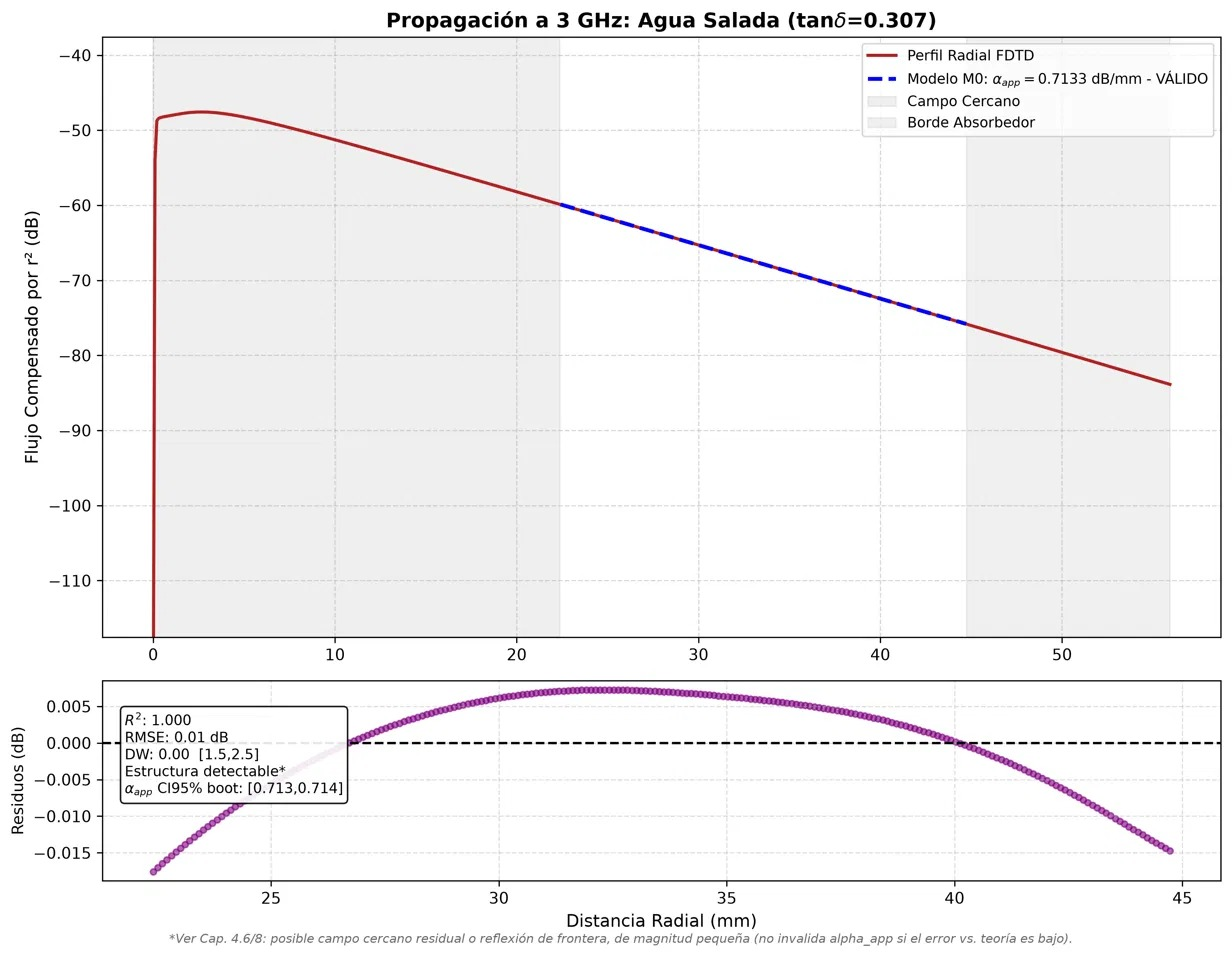
\includegraphics[width=0.83\linewidth]{figuras/Tesis_Resultado_agua_salada10px.jpeg}
\caption{Agua salada a 10 px/mm. Perfil radial y residuos de la atenuación ajustada.}\label{fig:anexo-agua-10}\end{figure}

\begin{figure}[htbp]\centering
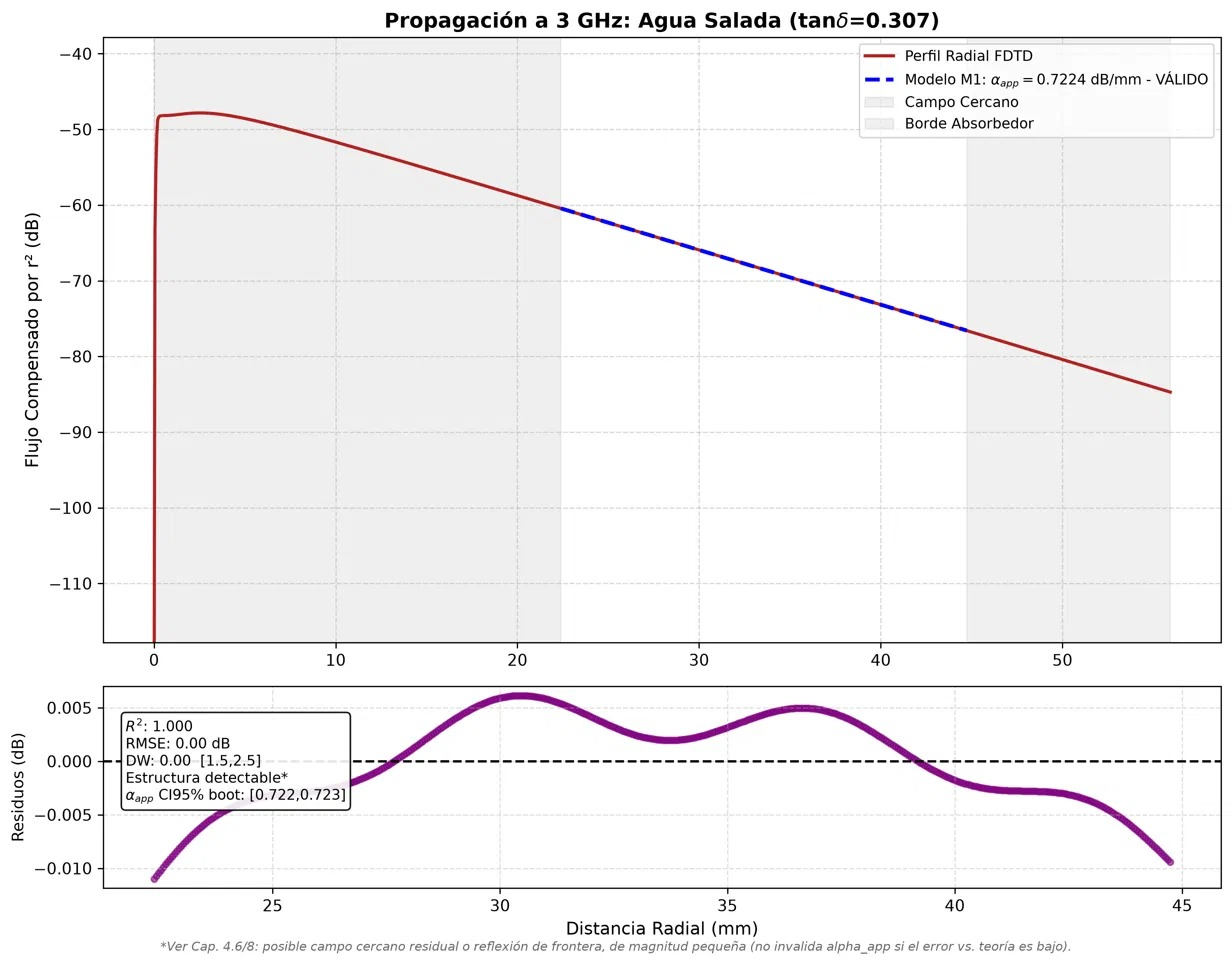
\includegraphics[width=0.83\linewidth]{figuras/Tesis_Resultado_agua_salada20px.jpeg}
\caption{Agua salada a 20 px/mm. Perfil radial y residuos de la atenuación ajustada.}\label{fig:anexo-agua-20}\end{figure}

\begin{figure}[htbp]\centering
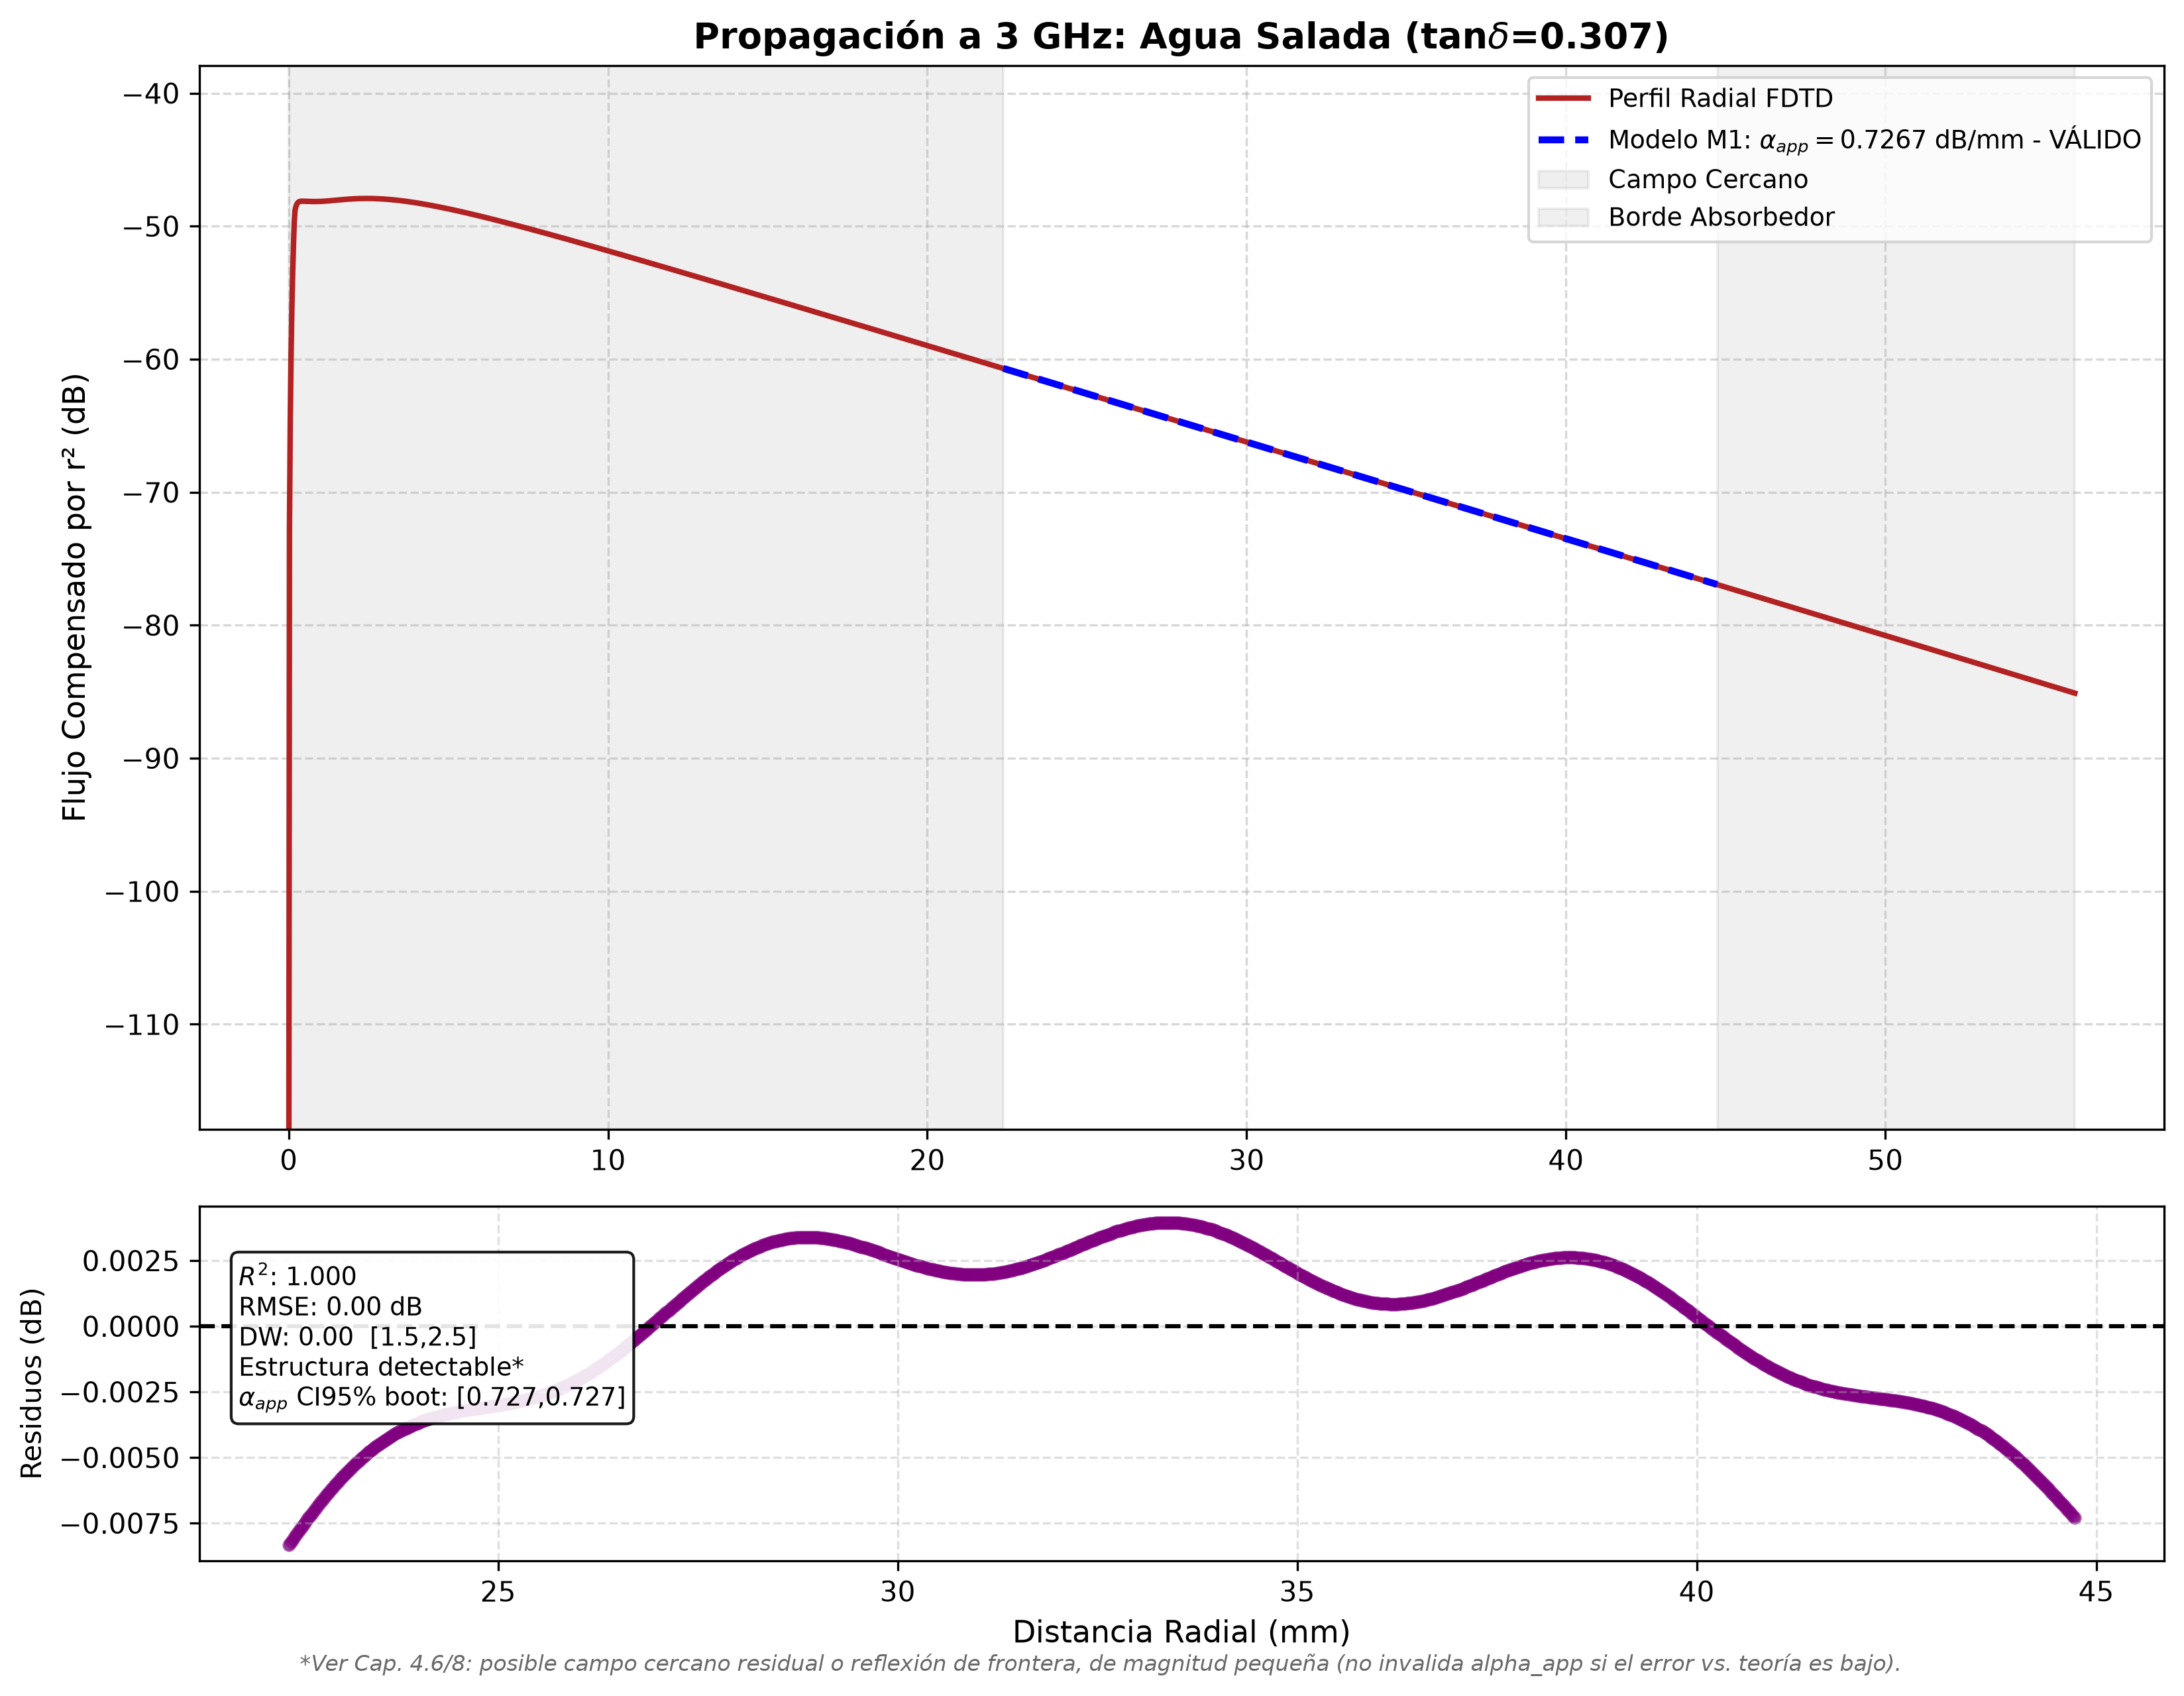
\includegraphics[width=0.83\linewidth]{figuras/Tesis_Resultado_agua_salada40px.png}
\caption{Agua salada a 40 px/mm. Perfil radial y residuos de la atenuación ajustada.}\label{fig:anexo-agua-40}\end{figure}

\begin{figure}[htbp]\centering
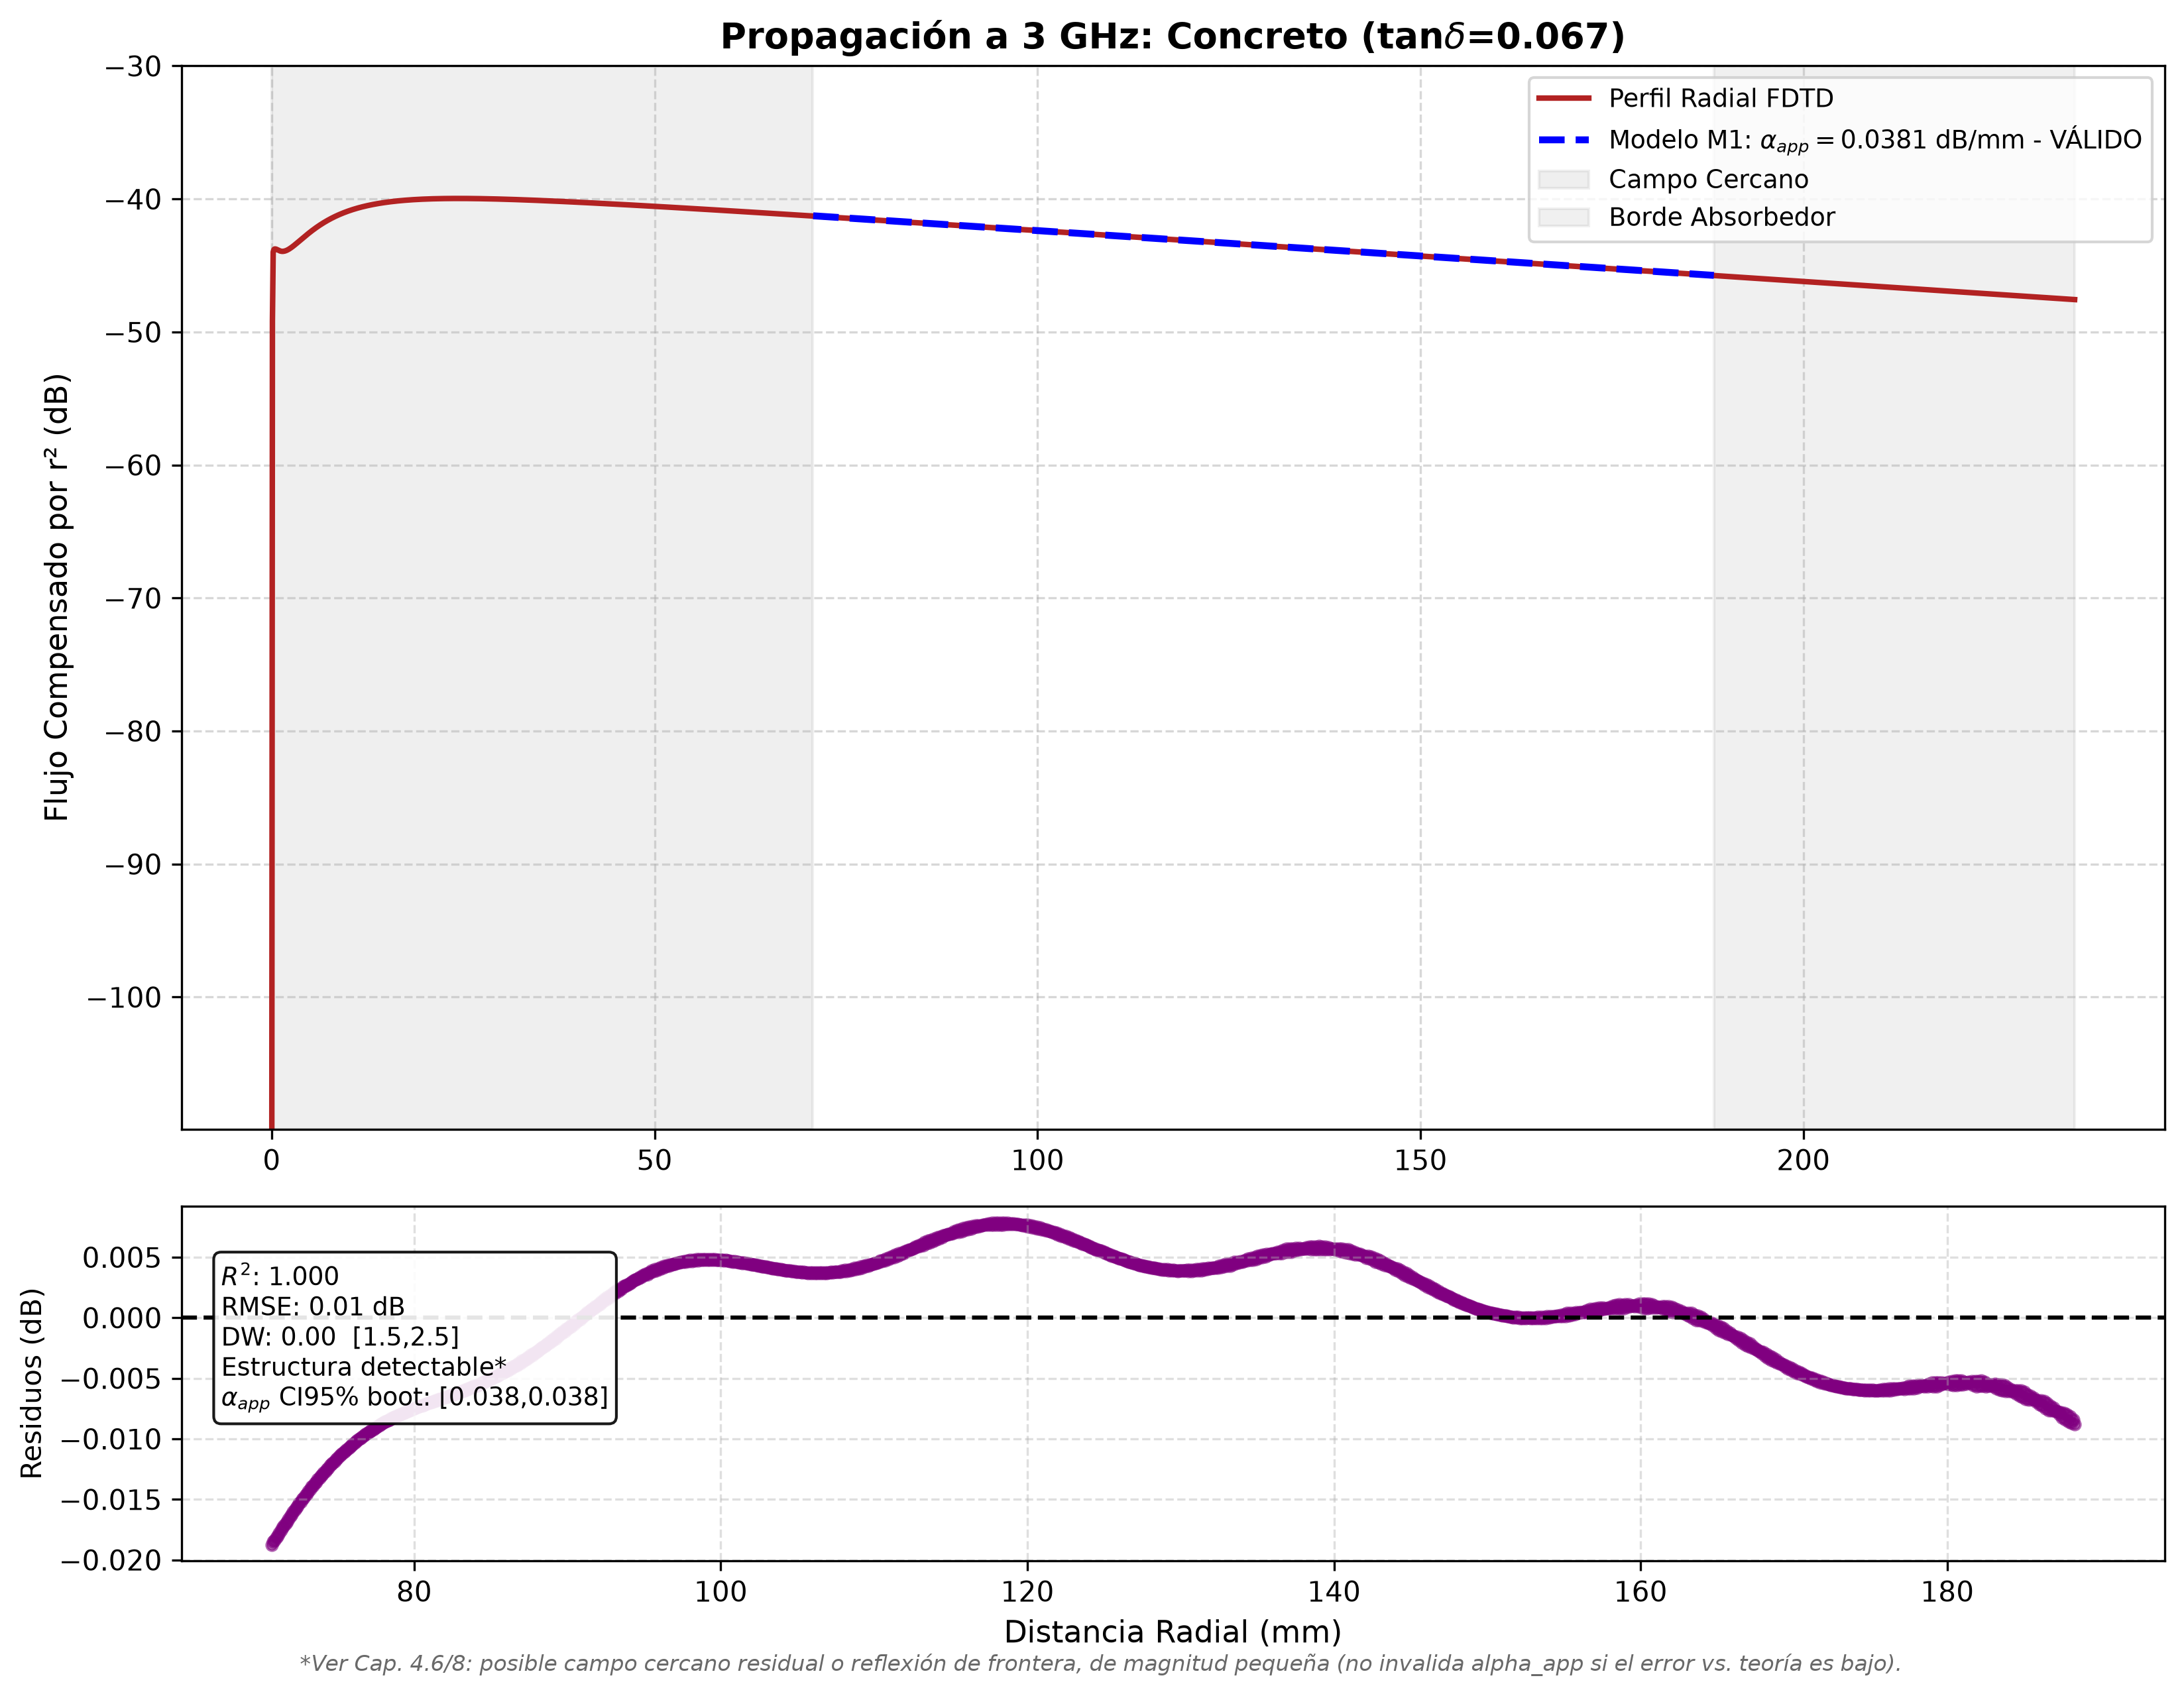
\includegraphics[width=0.83\linewidth]{figuras/Tesis_Resultado_concreto10px.png}
\caption{Concreto a 10 px/mm. Perfil radial y residuos de la atenuación ajustada.}\label{fig:anexo-concreto-10}\end{figure}

\begin{figure}[htbp]\centering
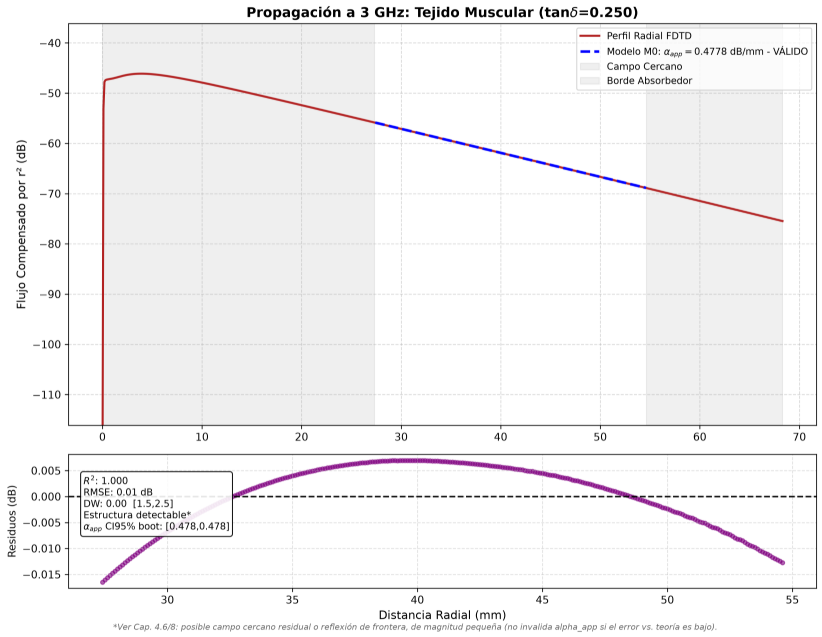
\includegraphics[width=0.83\linewidth]{figuras/Tesi_Resultados_tejido_mucular10px.png}
\caption{Tejido muscular a 10 px/mm. Perfil radial y residuos de la atenuación ajustada.}\label{fig:anexo-musculo-10}\end{figure}

\begin{figure}[htbp]\centering
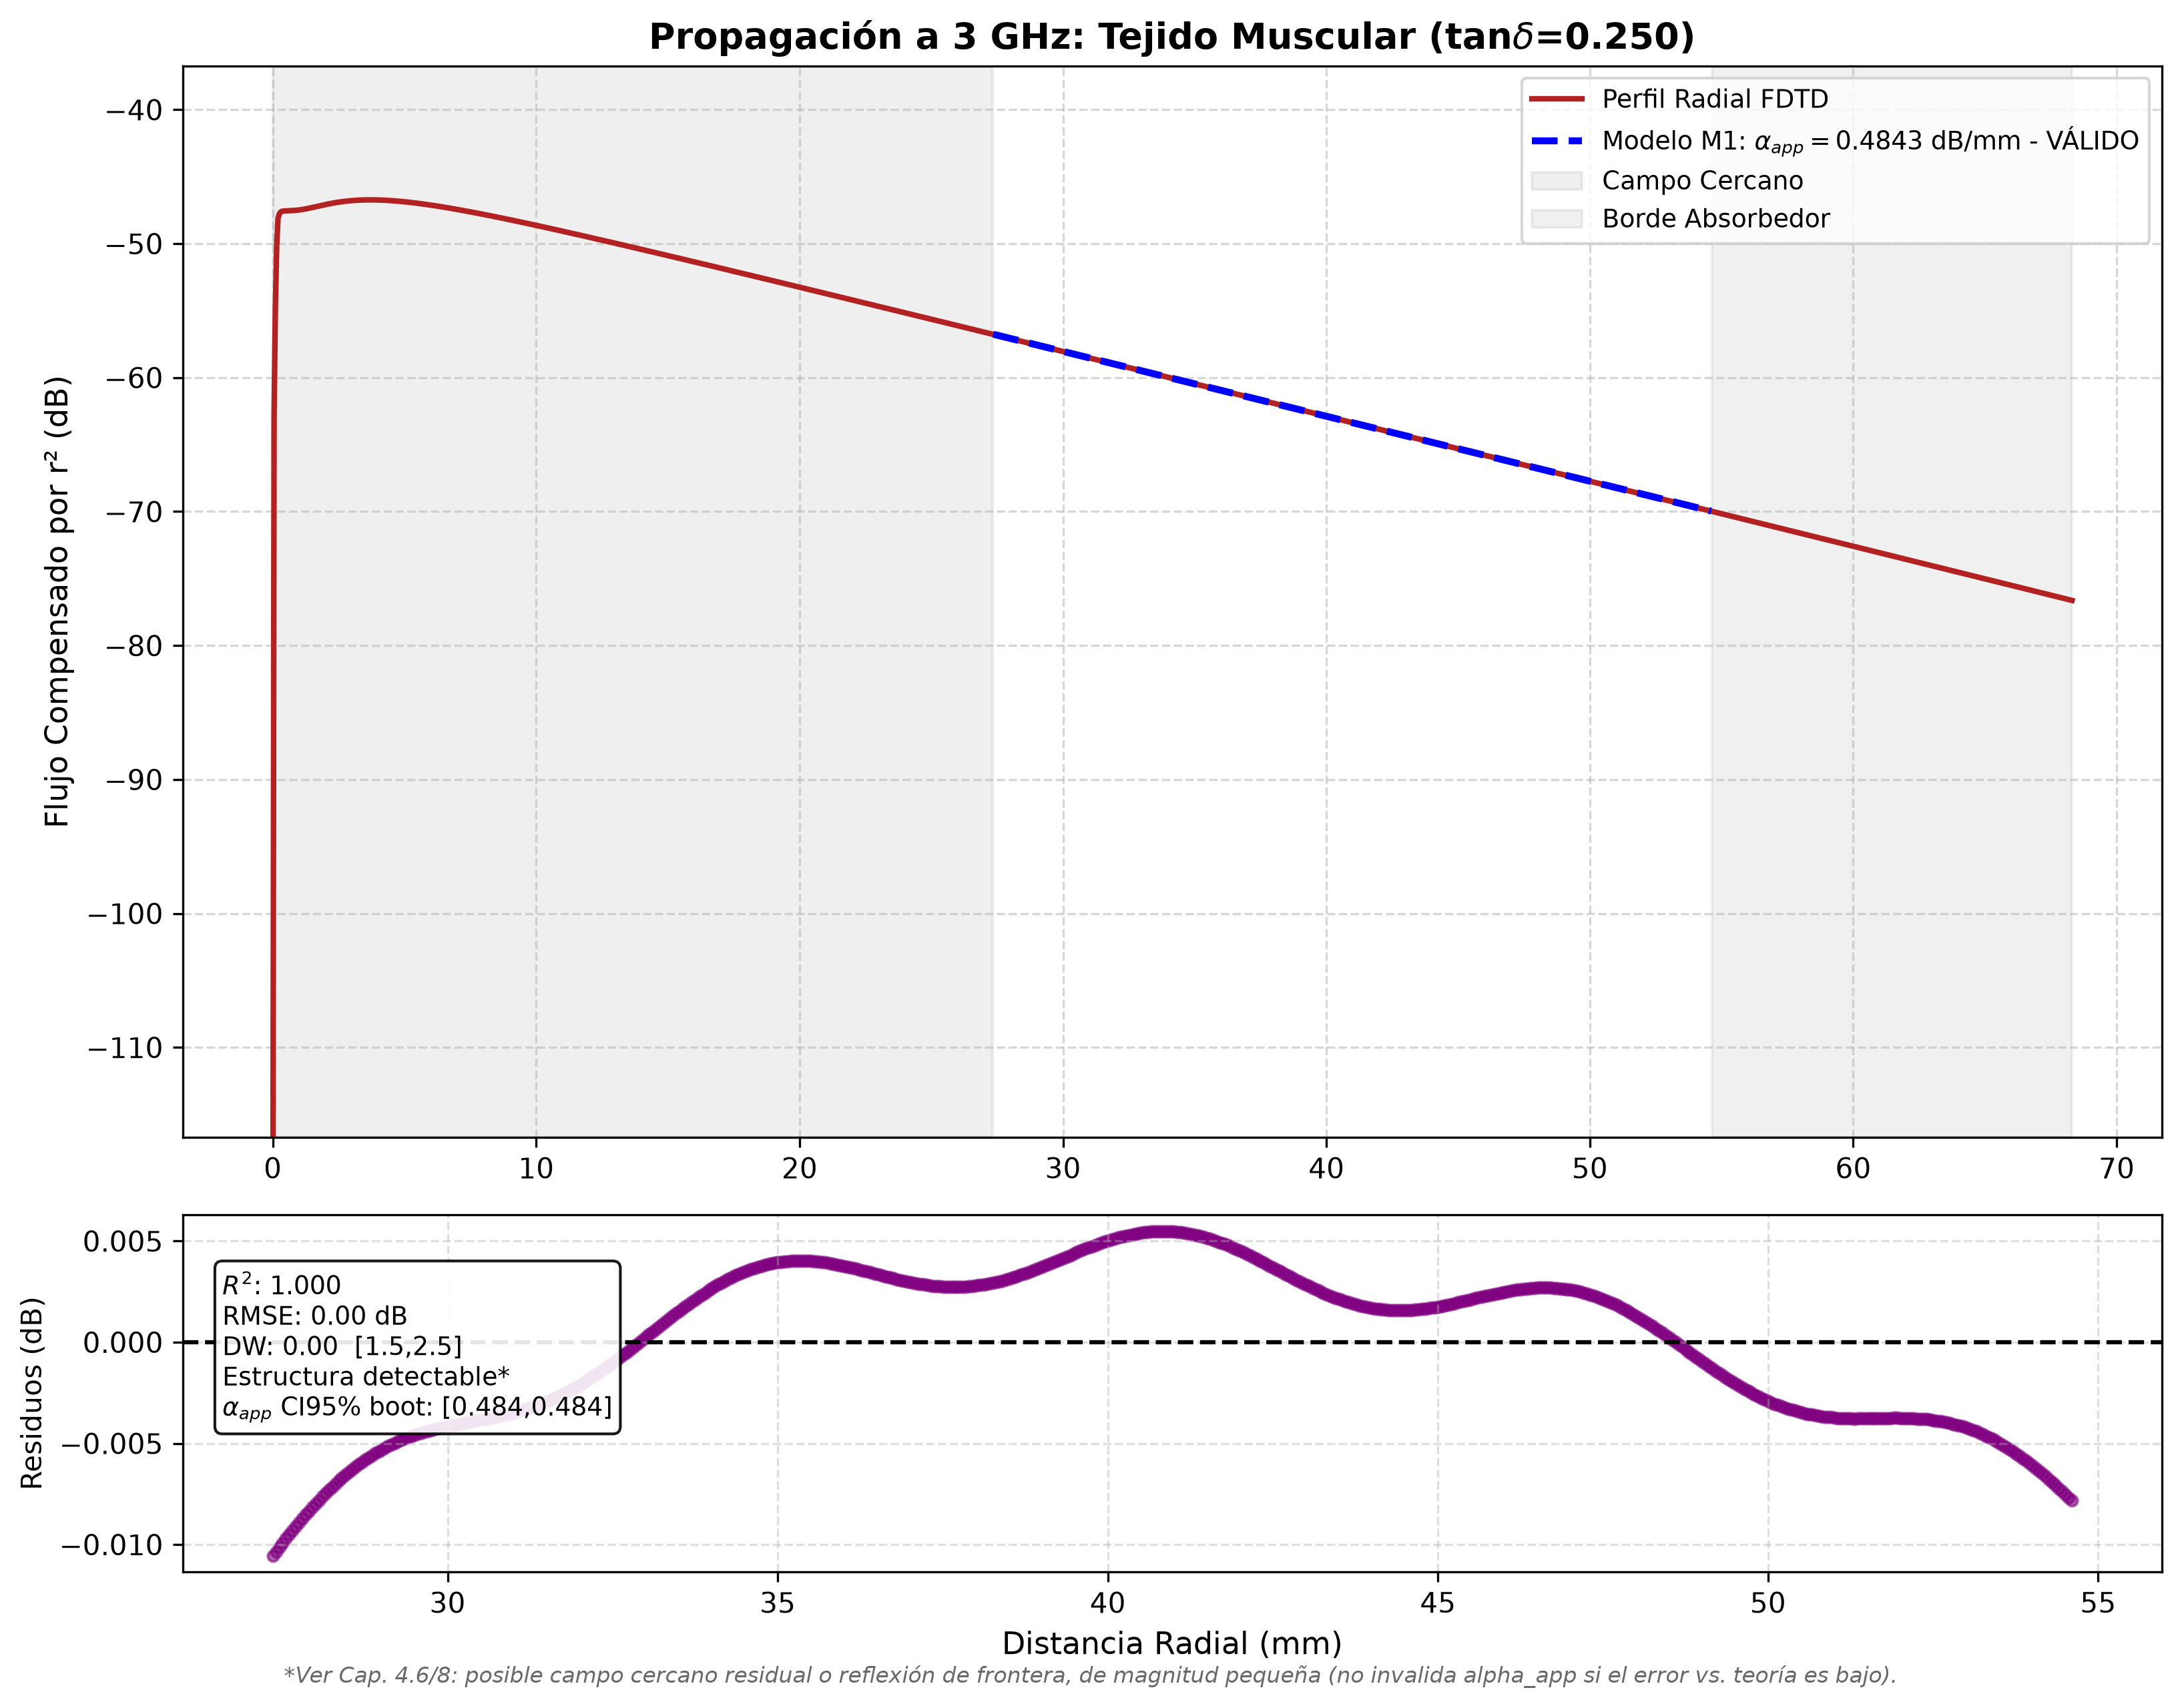
\includegraphics[width=0.83\linewidth]{figuras/Tesis_Resultado_tejido_muscular20px.png}
\caption{Tejido muscular a 20 px/mm. Perfil radial y residuos de la atenuación ajustada.}\label{fig:anexo-musculo-20}\end{figure}
